\chapter{Fundamentação Teórica}
\label{cap:fundamentacao-teorica}

Esta seção se dedica a fornecer o embasamento teórico necessário para a compreensão das
seções posteriores, focando principalmente no fluxo de processamento realizado por um
motor \textit{JavaScript}.

\section{\textit{JavaScript}}
\label{sec:javascript}

\textit{JavaScript} é uma linguagem de programação, que surgiu em 1995, criada pelo
desenvolvedor estadunidense, Brendan Eich, como parte do navegador
\textit{web Netscape Navigator} 2.0. O desenvolvimento da linguagem iniciou com o objetivo
de fazer com que o navegador tivesse a habilidade de interpretar \textit{scripts} e com
isso a criação de páginas \textit{web} dinâmicas. Ela apareceu em todos os navegadores
subsequentes da \textit{Netscape}, em todos os navegadores da Microsoft iniciando com o
\textit{Internet Explorer} 3.0, e desde 2002 tem sido suportada pelos navegadores mais
populares como \textit{Google Chrome}, \textit{Mozilla Firefox}, \textit{Apple Safari} e
\textit{Microsoft Internet Explorer}. \cite{w3cbs}

O desenvolvimento da padronização da linguagem foi iniciado em novembro de 1996 pela
\textit{Nestcape}, que ao finalizar submeteu a especificação a Assembléia Geral da ECMA
International, atualmente a maior autoridade da associação, que foi aceita e teve a
definição do padrão chamada de ECMAScript com a especificação ECMA-262 e ISO/IEC 16262
\cite{ecmascript}.

\subsection{Motor \textit{JavaScript}}
\label{ssec:jsengine}

Para que seja possível executar um \textit{script} feito na linguagem \textit{JavaScript},
é necessário que se tenha um motor \textit{JavaScript}, em inglês
\textit{JavaScript Engine}, que é responsável por interpretar e executar códigos da
linguagem. Embora existam vários usos para esse motor, ele é mais comumente utilizado em
navegadores, mas existem outros projetos como \textit{Node.js} que exercem esse trabalho
no lado do servidor.

Segundo definição apresentada no site da \textit{Mozilla Developer Network}, um motor
\textit{JavaScript} compila e executa \textit{scripts} contendo instruções e funções
escritos na linguagem \textit{JavaScript}, lida com a alocação de memória para os objetos
necessários para a execução dos \textit{scripts} e desalocação de memória dos objetos que
não são mais necessários. \cite{mdnjsapi}

Não há uma especificação formal que padronize o que um motor \textit{JavaScript} deve
possuir em sua implementação, entretanto alguns padrões podem ser percebidos nas
implementações existentes até então:

\begin{itemize}
    \item Analisador (Léxico + Sintático)
    \item Representação Intermediária
    \item Interpretador
    \item Compilador de linha de base
    \item Compilador de otimização
    \item Coletor de Lixo
\end{itemize}

O esquema lógico apresentado na Figura \ref{fig:image-1}, mostra o fluxo de processamento
feito pelo motor \textit{JavaScript}, executando em um processador multi-core, desde o
recebimento do código até sua execução.

\begin{figure}[h!]
    \centering
    \Caption{\label{fig:image-1} Esquema lógico sequencial de processamento de um motor \textit{JavaScript}}
    \UECEfig{}{
    \fbox{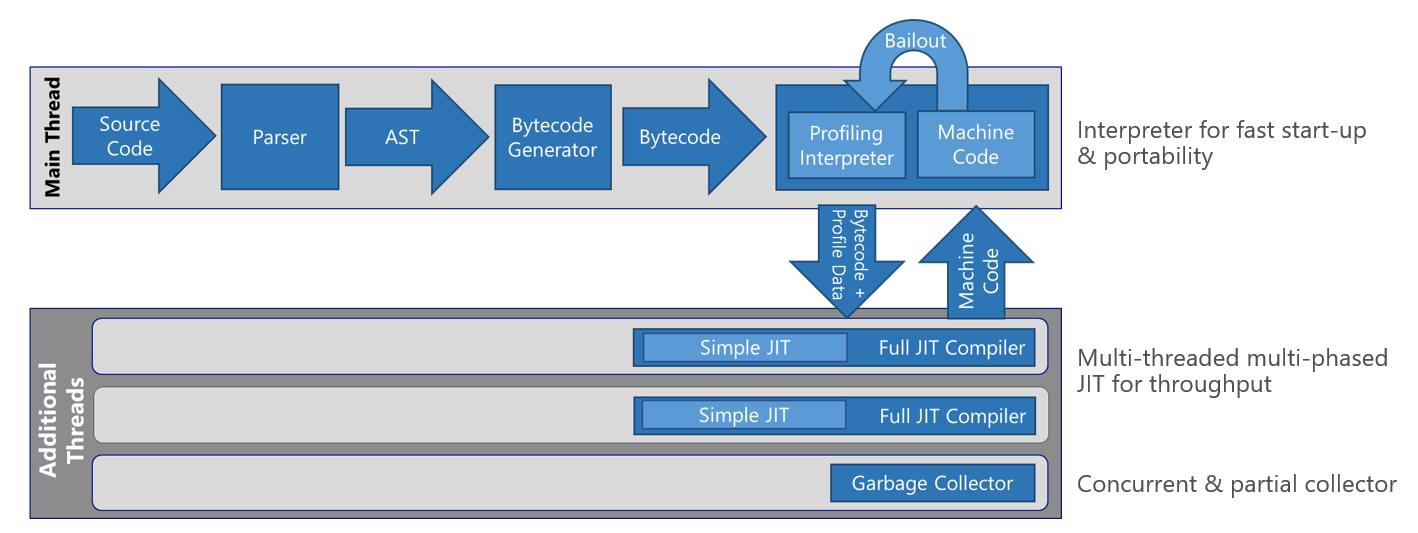
\includegraphics[width=14cm]{images/image-1}}
    }{
    \Fonte{\citeauthoronline{edgeengineopensource}}
    }
\end{figure}

Iniciando o processamento do código, como mostrado no esquema acima, será utilizado um
trecho de código que faz o cálculo do quadrado de um número e retorna o resultado desse
cálculo, como prova de conceito para mostrar passo a passo os resultados de cada etapa do
processo no motor \textit{JavaScript}. O trecho de código pode ser visto no Código-fonte
\ref{alg:code-1}.

\lstinputlisting[language=JavaScript,caption={\label{alg:code-1} \textit{Square} escrito em \textit{JavaScript}}]{code/square.js}

O motor ao receber o trecho de código inicia o \textit{parsing}, esse processo pode ser
dividido em dois subprocessos: Análise Léxica e Análise Sintática:

\begin{itemize}
    \item \textbf{Análise Léxica}: processo de quebrar uma entrada em uma sequência de
    símbolos (\textit{tokens}). \textit{Tokens} são o vocabulário linguístico: uma
    coleção de blocos de construção válidos, de acordo com uma gramática.
    \item \textbf{Análise Sintática}: processo de aplicação de regras de sintaxe, de
    acordo com uma gramática formal.
\end{itemize}

Cada um desses subprocessos possui um componente responsável por realizar tarefas
específicas de cada contexto, sendo eles:

\begin{itemize}
    \item \textbf{\textit{Lexer} ou \textit{Tokenizer}}: responsável por quebrar uma
    entrada em \textit{tokens} válidos, exercendo assim o papel de analisador léxico. O
    \textit{lexer} também sabe como tirar caminhos irrelevantes como espaços em branco e
    quebras de linha.
    \item \textbf{\textit{Parser}}: responsável pela construção da Árvore de Sintaxe
    Abstrata, em inglês \textit{Abtract Syntax Tree} (AST), analisando a estrutura do
    código de acordo com as regras de sintaxe da linguagem, buscando por possíveis erros
    baseado na escrita padrão da linguagem, para evitar erros durante a compilação ou
    resultados divergentes na execução do código ao final do processo.
\end{itemize}

O processo de \textit{parsing} é iterativo. O \textit{parser} solicita ao \textit{lexer}
um novo \textit{token}, e tenta combinar o \textit{token} recebido com uma das regras de
sintaxe. Se uma regra for correspondida, um novo nó correspondente ao \textit{token} é
adicionado a AST e o \textit{parser} solicitará o próximo \textit{token}, e assim
consecutivamente.

Se nenhuma regra corresponder, o \textit{parser} armazenará o \textit{token} internamente
e continuará pedindo \textit{tokens} até encontrar uma regra que corresponda a todos os
\textit{tokens} armazenados internamente. Se nenhuma regra for encontrada, que corresponda
aos \textit{tokens} armazenados, o \textit{parser} lançará uma exceção. Isso significa que o
código fornecido não é válido e possui erros de sintaxe.

Com base na função \textit{square} citada anteriormente, será obtido como resultado do
\textit{parsing} utilizando o primeiro subprocesso, \textit{tokenizer}
\footnote[1]{\textit{Tokenizer} pode ser compreendido como o processo de analisar uma
entrada de caracteres, como um código-fonte, e produzir uma sequência de símbolos que
podem ser manipulados mais facilmente por um \textit{parser}.}, os \textit{tokens} que
serão gerados e posteriormente analisados, cada um possuindo seu próprio tipo. Os
\textit{tokens} possem ser observados na Figura \ref{fig:image-2}.

\begin{figure}[h!]
    \centering
    \Caption{\label{fig:image-2} Resultado do \textit{Tokenizer} com base na função \textit{square}}
    \UECEfig{}{
    \fbox{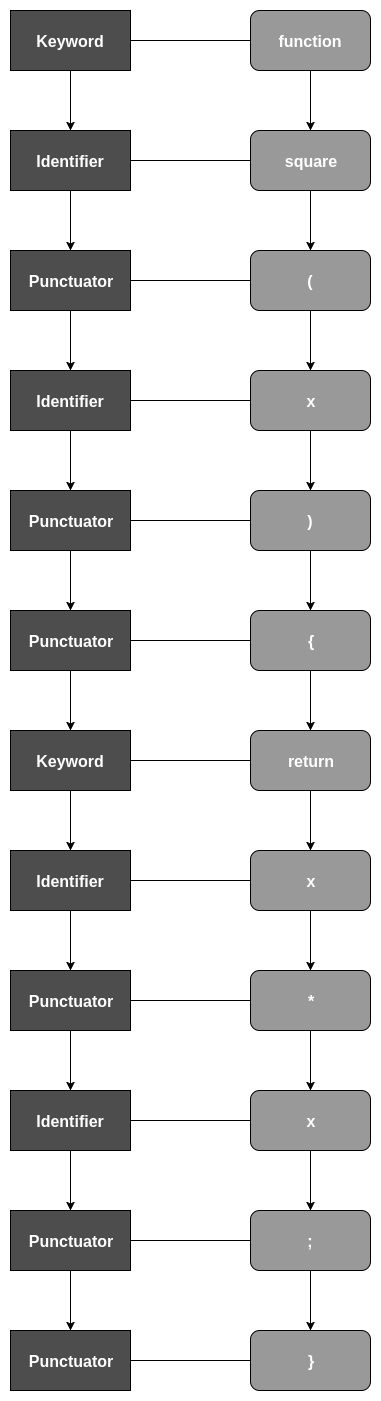
\includegraphics[width=4cm]{images/image-2}}
    }{
    \Fonte{Elaborada pelo autor.}
    }
\end{figure}

Após o resultado do \textit{tokenizer} ser gerado, uma Árvore de Sintaxe Abstrata, é
criada, para a função de potenciação conforme é mostrado na Figura \ref{fig:image-3}.

\begin{figure}[h!]
    \centering
    \Caption{\label{fig:image-3} Árvore de Sintaxe Abstrata gerada com base na função \textit{square}}
    \UECEfig{}{
    \fbox{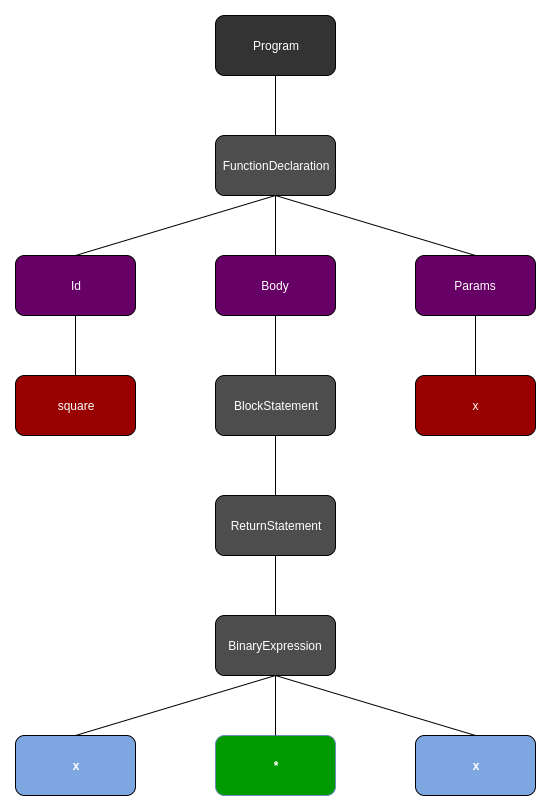
\includegraphics[width=8cm]{images/image-3}}
    }{
    \Fonte{Elaborada pelo autor.}
    }
\end{figure}

Após a geração da AST, com base na implementação do motor \textit{JavaScript}, o
\textit{bytecode generator} a converte para uma linguagem intermediária ou para código
nativo\footnote[2]{Conforme descrito acima, a etapa de geração do \textit{bytecode} pode
variar de acordo com a implementação do motor \textit{JavaScript}. Deixando a decisão de
utilizar ou não uma linguagem intermediária para o responsável pela implementação do
motor.}, e isso é feito para cada bloco de código representado na AST. Pode-se citar como
exemplo, alguns motores implementados até então:

\begin{itemize}
    \item \textbf{\textit{V8}}: implementado por um time da empresa Google e que é
    utilizado em seus navegadores, como \textit{Google Chrome} e \textit{Chromium}, que
    converte a AST diretamente para código nativo.
    \item \textbf{\textit{SpiderMonkey}}: o primeiro motor desenvolvido, criado pelo mesmo
    criador da linguagem \textit{JavaScript}, Brendan Eich, na Netscape e atualmente
    mantido pela Mozilla e que é utilizado em seus navegadores como
    \textit{Mozilla Firefox} e \textit{Firefox Nightly}, que converte a AST para uma
    linguagem intermediária.
    \item \textbf{\textit{Rhino}}: implementado e mantido por um time da empresa Mozilla,
    que por ser escrito utilizando a linguagem \textit{Java}, adiciona a etapa de tradução
    do código \textit{JavaScript} para classes \textit{Java}.
    \item \textbf{\textit{Chakra}}: implementado e mantido pela Microsoft, e que é
    utilizado no navegador \textit{Microsoft Edge}, que converte a AST para uma linguagem
    intermediária.
\end{itemize}

Códigos escritos em forma de \textit{bytecode} são formas canônicas de representação de
códigos que são utilizados pelos motores \textit{JavaScript}, são representações
intermediárias, que são projetadas para obter uma execução eficiente através de um
\textit{software} interpretador. Na Figura \ref{fig:image-4}, pode-se verificar o
\textit{bytecode} gerado, utilizando o motor \textit{SpiderMonkey}, para a função
\textit{square} utilizada como referência.

\begin{figure}[h!]
    \centering
    \Caption{\label{fig:image-4} Informações do \textit{bytecode} gerado com base na função \textit{square}}
    \UECEfig{}{
    \fbox{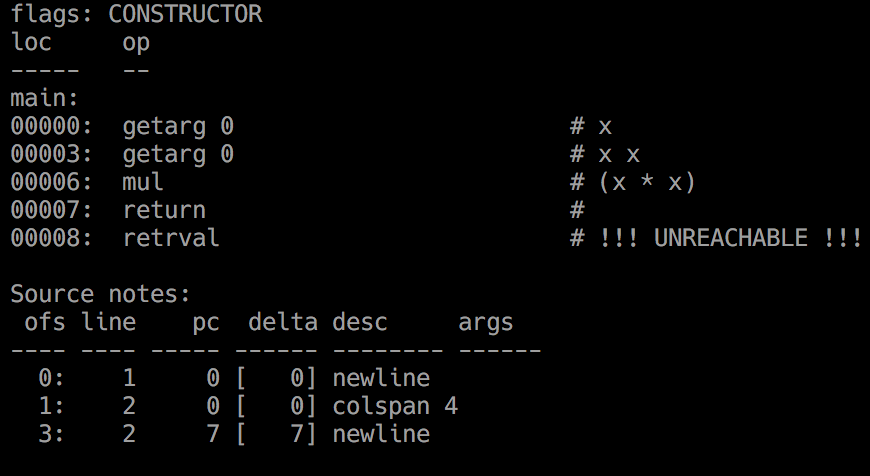
\includegraphics[width=10cm]{images/image-4}}
    }{
    \Fonte{Elaborada pelo autor.}
    \Nota{Informações obtidas utilizando a ferramenta \textit{JavaScript Shell} fornecida
    pelo motor \textit{SpiderMonkey}, usando internamente a função \textit{dis} da
    ferramenta.}
    }
\end{figure}

Após o \textit{bytecode} ter sido gerado, passa-se para a etapa de interpretação e
execução da representação intermediária, que é feita processando uma instrução por vez
percorrendo o \textit{bytecode} gerado. Quando o \textit{bytecode} chega até a área de
execução, observa-se a existência de dois componentes importantes para a performance de um
motor \textit{JavaScript}, que são o JIT (\textit{Just-in-Time Compiler}) e o Coletor de
Lixo (\textit{Garbage Collector}).

JIT, ou \textit{Just-in-Time compiler}, é o responsável por fazer a tradução de
\textit{bytecode} para código de máquina durante a execução do programa, ou seja, assim
que um trecho de código é solicitado, o JIT faz a transformação do \textit{bytecode} para
código de máquina, referente ao bloco solicitado e o disponibiliza para execução, fazendo
com que a disponibilização do resultado seja rápida e não consuma ciclos de processamento
desnecessários, entregando somente os blocos que serão utilizados no momento em que forem
solicitados.

O outro componente importante é o Coletor de Lixo, que é a área responsável pelo
gerenciamento automático da memória que é ocupada por objetos, sendo denominados como
"lixo" as posições de memória que estão sendo ocupadas com informações referentes ao
programa em execução, mas que não são relevantes ou que não estão sendo utilizadas.

Ambos os componentes comentados anteriormente, JIT e Coletor de Lixo, são executados
quando existe uma solicitação de um trecho de código \textit{JavaScript}, e estão
disponíveis durante toda a execução do motor \textit{JavaScript}, por isso estão
diretamente ligados ao passo de execução dentro do processo de interpretação de um código
\textit{JavaScript}.

Entretanto, no V8, que não utiliza uma representação intermediária, esse processo é um
pouco diferente. Ele utiliza dois compiladores, que podem ser denominados como o
compilador simples e o otimizador. O compilador simples é um compilador que não tem foco
em otimização, apesar de ainda assim realizar algumas, tem como principal objetivo
produzir código nativo tão rápido quanto possível, o que é importante para manter os
tempos de carregamento de uma página rápidos. \textit{Crankshaft}, e o atual
\textit{TurboFan}, são exemplos de compiladores com foco em otimização, também conhecidos
como otimizadores. O \textit{V8} compila todo o código com o compilador simples e em seguida
utiliza um \textit{profiler}\footnote[1]{\textit{Profiling} é uma forma de análise de
código dinâmica, que mede por exemplo, a complexidade espacial ou temporal de um algoritmo
específico, ou a frequência e duração de chamadas de funções. Comumente, um
\textit{profiler} serve para auxiliar a otimização de aplicações, selecionando quais
trechos de código darão um maior desempenho se otimizadas.} interno para selecionar as
funções a serem otimizadas, na maioria dos casos são as funções mais acessadas ou com
maior custo de processamento, pelo otimizador.

\section{\textit{WebAssembly}}
\label{sec:webassembly}

De acordo com a definição encontrada na especificação, ainda em desenvolvimento, do
\textit{WebAssembly}, é descrito que ele é um formato de código seguro, portátil e de
baixo nível projetado para uma execução eficiente e que possui uma representação compacta.
O objetivo principal é permitir que aplicações de alto desempenho sejam executados na
\textit{web}, mas não faz quaisquer pressupostos específicos da \textit{web} ou requer
quaisquer recursos específicos da \textit{web}, sendo assim pode ser empregado em outros
ambientes. \textit{WebAssembly} é um padrão aberto desenvolvido por um grupo comunitário
da W3C (\textit{World Wide Web Consortium})
\footnote[2]{\url{https://www.w3.org/community/webassembly/}} que inclui representantes de
todos os principais fornecedores de navegadores. A especificação descreve a versão 1.0 do
padrão central do \textit{WebAssembly}, e pretende-se que seja substituído por novos
lançamentos incrementais com recursos adicionais no futuro. \cite{wa}

\textit{WebAssembly} é a primeira solução para a execução de código de baixo nível na
\textit{web} que oferece todos os objetivos abaixo. É o resultado de uma colaboração sem
precedentes entre os principais fornecedores de navegadores e um grupo comunitário on-line
para construir uma solução comum para aplicativos de alto desempenho. \cite{wapaper}

Segundo a atual especificação, o \textit{WebAssembly} possui alguns objetivos principais
em sua modelagem:

\begin{itemize}
    \item Semântica rápida, segura e portátil:
    \begin{itemize}
        \item \textbf{Rápido}: execução com o desempenho próximo do código nativo,
        aproveitando as capacidades comuns a todos os \textit{hardwares} contemporâneos.
        \item \textbf{Seguro}: código validado e executado em um ambiente autocontido e
        seguro no que se refere a memória, impedindo a corrupção de dados ou violações de
        segurança.
        \item \textbf{Bem definido}: define de forma completa e precisa programas válidos
        e seu comportamento, de forma que seja fácil argumentar formalmente e/ou
        informalmente.
        \item \textbf{Independente de \textit{Hardware}}: código pode ser compilado em
        todas as arquiteturas modernas, dispositivos \textit{desktop} ou móveis e em
        sistemas integrados.
        \item \textbf{Independente de linguagem}: não privilegia nenhuma linguagem,
        modelo de programação ou modelo de objeto específico.
        \item \textbf{Independente de plataforma}: pode ser incorporado em navegadores,
        pode ser executado como uma VM autônoma ou integrado em outros ambientes.
        \item \textbf{Aberto}: programas podem interoperar com seu ambiente de forma
        simples e universal.
    \end{itemize}
    \item Representação eficiente e portátil:
    \begin{itemize}
        \item \textbf{Compacto}: possui um formato binário que é mais rápido de ser
        transmitido, sendo menor que os formatos de texto típicos ou os formatos de
        código nativo.
        \item \textbf{Modularizado}: aplicações podem ser divididas em partes menores que
        podem ser transmitidas, armazenadas em \textit{cache} e consumidas separadamente.
        \item \textbf{Eficiente}: pode ser decodificado, validado e compilado em uma única
        passagem rápida, igualmente como é feito com compilação \textit{just-in-time}
        (JIT) ou \textit{ahead-of-time} (AOT).
        \item \textbf{Fluido}: permite que os processos de decodificação, validação e
        compilação sejam iniciados o mais rápido possível, antes de todos os dados serem
        recebidos.
        \item \textbf{Paralelizável}: permite que os processos de decodificação, validação
        e compilação sejam divididos em muitas tarefas paralelas independentes.
        \item \textbf{Portável}: não faz nenhum pressuposto de arquitetura que não seja
        amplamente suportada por um \textit{hardware} moderno.
    \end{itemize}
\end{itemize}

Além disso, o \textit{WebAssembly} também se destina a ser fácil de inspecionar e depurar,
especialmente em ambientes como navegadores \textit{web}, mas esses recursos não serão
tratados na especificação atual. \cite{wa}

Antes de prosseguir, é necessário que se tenha conhecimento de alguns conceitos-chave
sobre \textit{WebAssembly}, pois serão necessários para entender seu fluxo de
processamento posteriormente:

\begin{itemize}
    \item \textbf{Módulo}: aplicações \textit{WebAssembly} são organizadas em módulos, que
    são a unidade básica de implantação, carregamento e compilação. Um módulo contém
    definições de tipos, funções, tabelas, memórias e variáveis globais. Além disso, pode
    declarar importações e exportações e fornecer lógica de inicialização na forma de
    segmentos de dados\footnote[1]{O conteúdo inicial de uma memória são \textit{bytes}
    "zero". O componente de dados de um módulo, \textit{data}, define um vetor de dados
    que inicializa um intervalo de memória em um determinado deslocamento com um vetor
    estático de \textit{bytes}.} e elementos\footnote[2]{O conteúdo inicial de uma tabela
    não está inicializada. O componente de elementos de um módulo, \textit{elem}, define
    um vetor de elementos que inicializa um intervalo de uma tabela em um determinado
    deslocamento com um vetor estático de elementos.} ou uma função de início.
    \item \textbf{Funções}: o código interno de um módulo é organizado em funções
    individuais. Cada função possui uma sequência de valores como parâmetros e retorna uma
    sequência de valores como resultado, conforme definido pelo seu tipo de função.
    \item \textbf{Instruções}: o processamento de um código \textit{WebAssembly} é baseado
    em uma máquina de pilha. O código de uma função consiste em uma sequência de
    instruções que manipulam valores em uma pilha de operandos implícita, desempilhando
    valores de argumentos e empilhando valores de resultados. No entanto, graças ao
    sistema de tipos, o leiaute da pilha de operandos pode ser determinado de forma
    estática em qualquer ponto do código, de modo que as implementações reais possam
    compilar o fluxo de dados entre as instruções diretamente sem nunca materializar a
    pilha de operandos. A organização da pilha é meramente uma maneira de conseguir uma
    representação compacta do programa, foi escolhido esse modelo pois se mostrou menor do
    que uma máquina registradora.
    \item \textbf{Memória}: o armazenamento principal de um módulo \textit{WebAssembly} é
    um grande vetor de \textit{bytes}, funcionando com uma memória linear. O tamanho do
    vetor sempre é um múltiplo do tamanho da página, páginas são subdivisões da memória
    para permitir-lhe uma utilização mais eficiente. Os \textit{bytes} podem ser
    manipulados através de instruções de memória, a execução de um segmento de dados, ou
    por meios externos fornecidos por quem está acoplando o \textit{WebAssembly}, um motor
    \textit{JavaScript} ou um sistema operacional por exemplo, que pode ser chamado de
    \textit{embedder}.
    \item \textbf{Exceções}: algumas instruções podem produzir um erro inesperado, que
    imediatamente aborta o processamento atual. As exceções atualmente não podem ser
    manipuladas por um código \textit{WebAssembly}, mas o \textit{embedder} normalmente
    fornecerá meios para lidar com essa condição. Se um código \textit{WebAssembly} for
    utilizado por um motor \textit{JavaScript} e ocorrer um erro interno, será lançada uma
    exceção \textit{JavaScript} contendo um \textit{stacktrace} com uma pilha de chamadas
    \textit{JavaScript} e \textit{WebAssembly}, que poderá ser manipulado por um código
    \textit{JavaScript}.
\end{itemize}

\subsection{Compilador}
\label{ssec:wa-compiler}

Quando se envia um código para ser executado na máquina de um usuário na \textit{web}, não
se sabe qual será a arquitetura de destino em que o código será executado. Então, o
\textit{WebAssembly} é um pouco diferente de outros tipos de \textit{assembly}. É um
idioma de máquina para uma máquina conceitual, e não para uma máquina física real, pode-se
dizer então que instruções \textit{WebAssembly} são instruções virtuais. Essas instruções
têm um mapeamento muito mais direto para o código de máquina do que o código-fonte
\textit{JavaScript}. Eles representam uma espécie de interseção do que pode ser feito de
forma eficiente em todo o \textit{hardware} popular comum, mas eles não são mapeamentos
diretos para o código de máquina específico de um \textit{hardware} específico. Pode-se
ver isso na Figura \ref{fig:image-5}.

\begin{figure}[h!]
    \centering
    \Caption{\label{fig:image-5} Processo de compilação de um código \textit{WebAssembly}}
    \UECEfig{}{
    \fbox{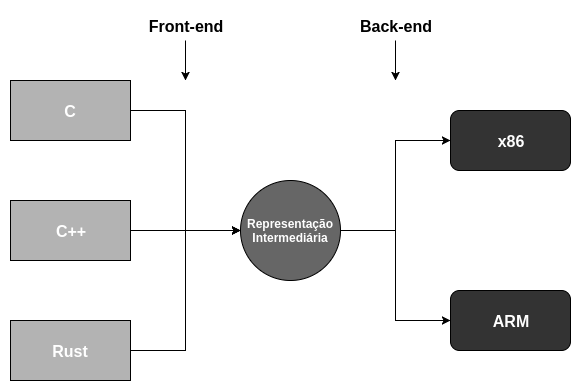
\includegraphics[width=10cm]{images/image-5}}
    }{
    \Fonte{Elaborada pelo autor.}
    }
\end{figure}

Até então, o projeto que possui maior suporte a \textit{WebAssembly} é o LLVM,
\textit{Low Level Virtual Machine}, que é uma infraestrutura de compilação, em que,
segundo Lattner, fornece componentes modulares e reutilizáveis para a construção de
compiladores, que auxiliam na redução de custo e tempo na criação de um compilador
particular. Essa infraestrutura possui uma representação intermediária própria, além
de diversas bibliotecas e componentes com interfaces bem definidas e ferramentas
construídas pelas próprias bibliotecas. LLVM fornece componentes totalmente independentes
de linguagem e máquina alvo, permitindo assim, que algoritmos de diferentes linguagens
possam ser conectados e otimizados em conjunto. \cite{llvm-intro}

LLVM é baseado na forma de atribuição única estática, em inglês
\textit{Static Single Assignment form} (SSA), que conforme Lattner e Adve, fornece
segurança de tipo, operações de baixo nível, flexibilidade e a capacidade de representar
todas as linguagens de alto nível de forma simples. A forma SSA é uma propriedade de uma
representação intermediária em que cada variável é atribuída exatamente uma vez, e cada
variável é definida antes de ser utilizada. \cite{llvm-langref}

Supondo que queira-se ir de \textit{C} para \textit{WebAssembly}, pode ser utilizado o
\textit{front-end} clang\footnote[1]{\url{https://clang.llvm.org}} para passar de
\textit{C} para a representação intermediária do LLVM. Uma vez que se está na RI do LLVM,
ele o entende, e então pode executar algumas otimizações. Para ir da RI do LLVM para o
\textit{WebAssembly}, é preciso um \textit{back-end}. Existe um que está atualmente em
andamento no projeto LLVM, e está com a sua maior parte implementada e deve ser finalizado
em breve. No entanto, ainda não é possível utilizá-lo. Existe outra ferramenta chamada
\textit{Emscripten}, que possui o seu próprio \textit{back-end} que pode produzir
\textit{WebAssembly} compilando para outra representação, denominada \textit{asm.js}, e em
seguida, convertendo-o para \textit{WebAssembly}. Pode-se ver isso na Figura
\ref{fig:image-6}.

\begin{figure}[h!]
    \centering
    \Caption{\label{fig:image-6} Ferramenta de compilação}
    \UECEfig{}{
    \fbox{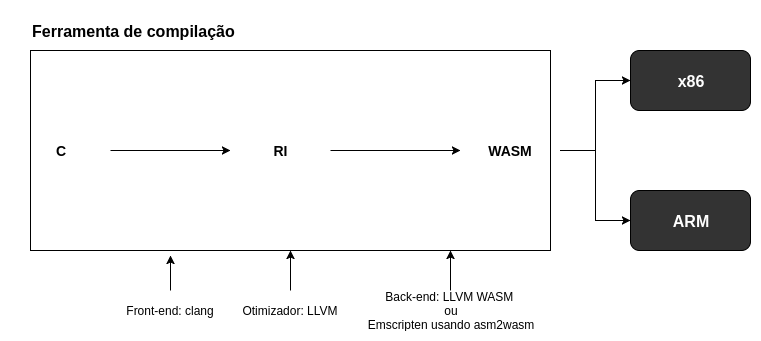
\includegraphics[width=12cm]{images/image-6}}
    }{
    \Fonte{Elaborada pelo autor.}
    }
\end{figure}

\subsection{Representação Intermediária}
\label{ssec:wa-ir}

Para permitir que o \textit{WebAssembly} seja lido e editado mais facilmente, existe uma
representação textual, além da representação binária (\textit{WASM}) citada anteriormente,
o \textit{WAST}. É um formato intermediário projetado para ser utilizado em editores de
texto, ferramentas de desenvolvimento, e até mesmo em navegadores.

Em ambos os formatos, binário e textual, a unidade fundamental de um código
\textit{WebAssembly} é um módulo. No formato de texto, um módulo é representado como uma
grande expressão em S. As expressões \textit{S} são um formato textual muito antigo e
muito simples para representar árvores, e assim pode-se pensar em um módulo como uma
árvore de nós que descrevem a estrutura do módulo e seu código. Ao contrário da árvore de
sintaxe abstrata de uma linguagem de programação, a árvore de um código
\textit{WebAssembly} é bastante plana, principalmente composta por listas de instruções.
Pode-se ver um exemplo no Código-fonte \ref{alg:code-2}.

\lstinputlisting[language=Lisp,caption={\label{alg:code-2} Exemplo de um módulo na representação intermediária textual}]{code/module.cl}

Todo o código em um módulo \textit{WebAssembly} é agrupado em funções, que possuem a
seguinte estrutura de pseudo-código:

\lstinputlisting[language=Lisp,caption={\label{alg:code-3} Estrutura de uma expressão \textit{S}}]{code/module-signature.cl}

\begin{itemize}
    \item \textbf{\textit{Signature}}: declara o que a função requer (parâmetros) e
    retorna (valores de retorno).
    \item \textbf{\textit{Locals}}: são definições de variáveis com tipos explícitos
    declarados.
    \item \textbf{\textit{Body}}: é apenas uma lista linear de instruções de baixo nível.
\end{itemize}

O formato textual também pode ser utilizado para simplificar a criação de um compilador
de uma linguagem específica para \textit{WebAssembly}, pois basta o novo compilador
suportar a representação textual e posteriormente utilizar um outro compilador que utilize
essa representação textual para a representação binária.

\subsection{Fluxo de processamento de um código \textit{WebAssembly}}
\label{ssec:wa-flow}

O esquema lógico apresentado na Figura \ref{fig:image-7} mostra o fluxo de processamento
de um código \textit{WebAssembly}, desde a compilação até sua execução, destacando as
etapas mais significativas para a explicação.

\begin{figure}[h!]
    \centering
    \Caption{\label{fig:image-7} Esquema lógico sequencial de processamento de um código \textit{WebAssembly}}
    \UECEfig{}{
    \fbox{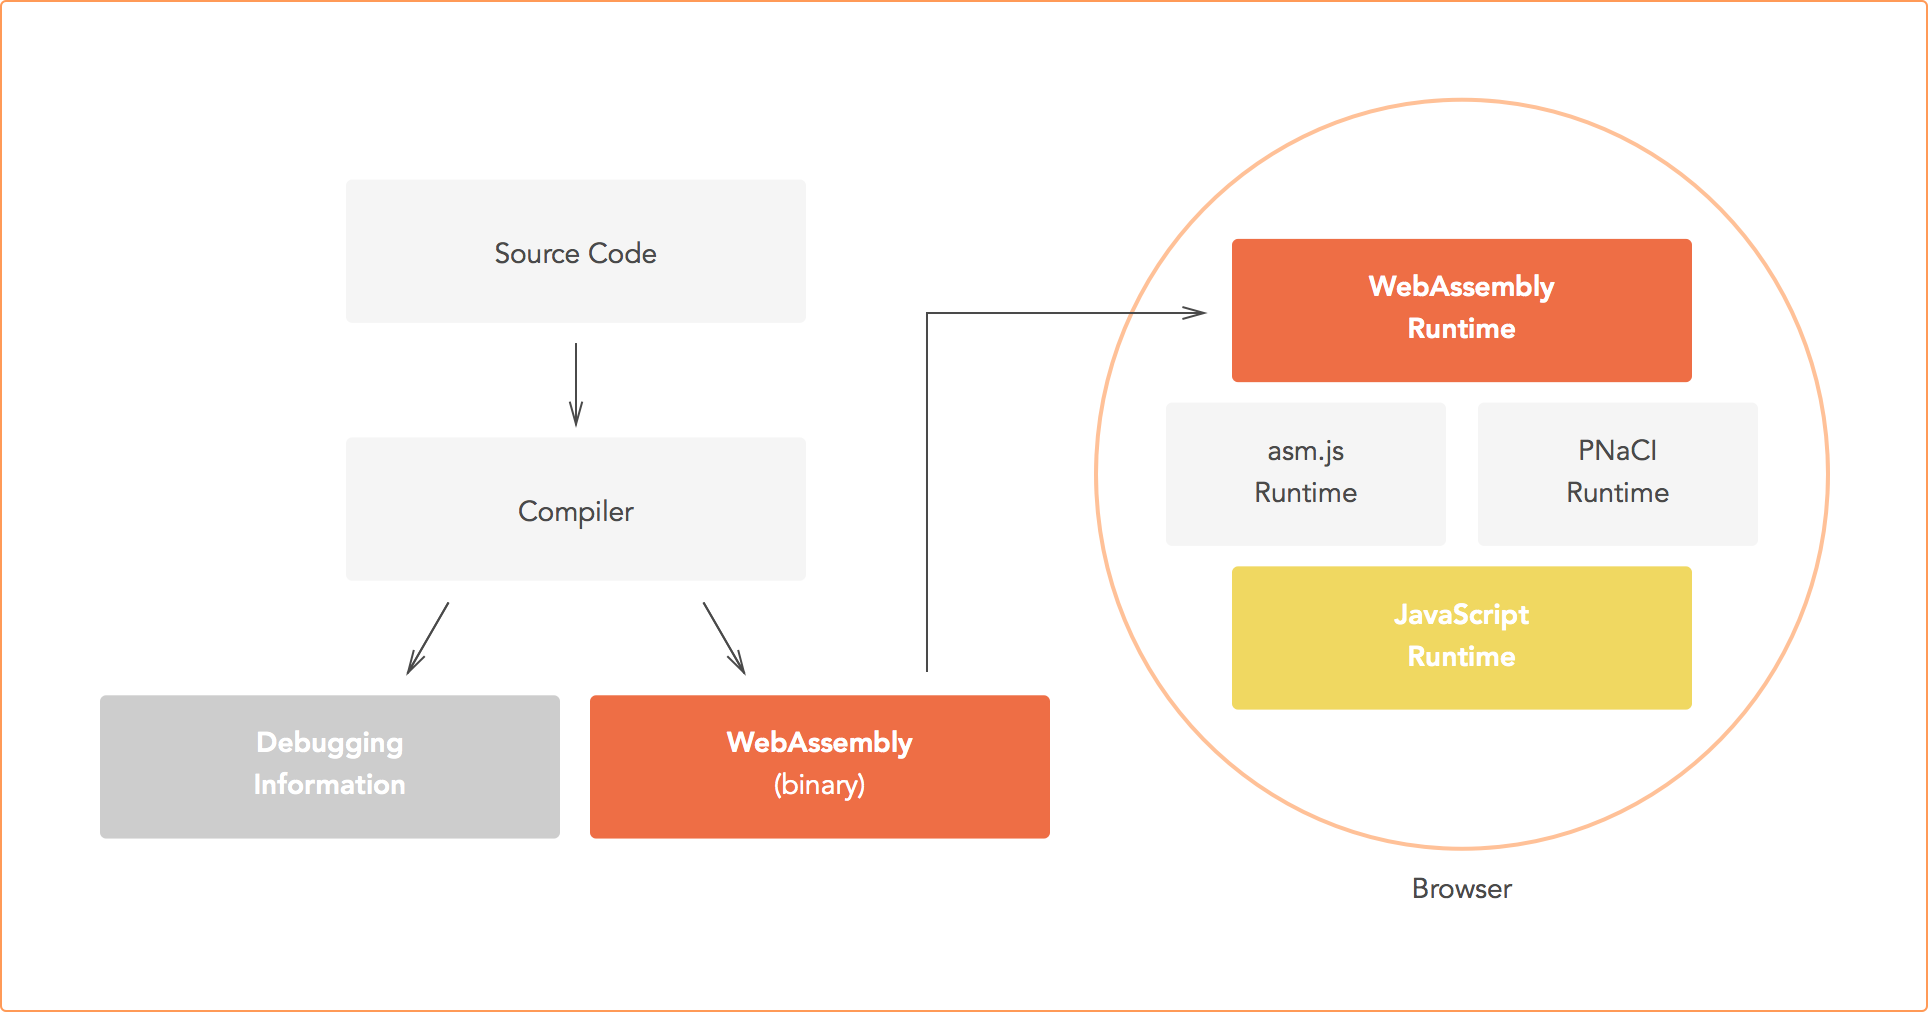
\includegraphics[width=12cm]{images/image-7}}
    }{
    \Fonte{\citeauthoronline{wa-things}}
    }
\end{figure}

Iniciando o processamento do código, conforme mostrado no esquema acima, será utilizada a
mesma função utilizada na seção anterior, alterando apenas a linguagem, \textit{C}, que
executa o cálculo do quadrado de um número e retorna o resultado desse cálculo, como prova
de conceito para mostrar passo a passo os resultados de cada etapa do processo realizado
pelo motor \textit{JavaScript}. O trecho de código pode ser visto no Código-fonte
\ref{alg:code-4}.

\lstinputlisting[language=C,caption={\label{alg:code-4} \textit{Square} escrito em \textit{C}}]{code/square.c}

Se for adicionado nesse processo a etapa de compilar a função \textit{square}, escrita em
\textit{C}, para a representação intermediária textual de \textit{WebAssembly}, serão
obtidos como saída as expressões \textit{S} exibidas na Figura \ref{fig:image-8}.

\begin{figure}[h!]
    \centering
    \Caption{\label{fig:image-8} Representação intermediária textual da função \textit{square}}
    \UECEfig{}{
    \fbox{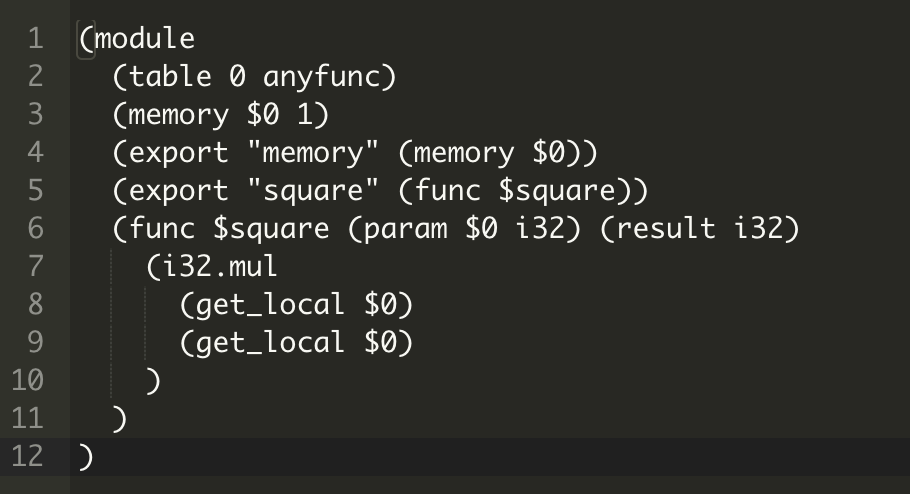
\includegraphics[width=12cm]{images/image-8}}
    }{
    \Fonte{Elaborada pelo autor.}
    \Nota{Expressões \textit{S} que representam a função \textit{square}.}
    }
\end{figure}

A próxima etapa é compilar da representação intermediária textual para a representação
intermediária binária, que é o formato que será utilizado durante a execução pelo motor
JavaScript. Pode-se observar a saída dessa etapa, onde é exibida a representação binária
da função \textit{square} na Figura \ref{fig:image-9}.

\begin{figure}[h!]
    \centering
    \Caption{\label{fig:image-9} Representação intermediária binária da função \textit{square}}
    \UECEfig{}{
    \fbox{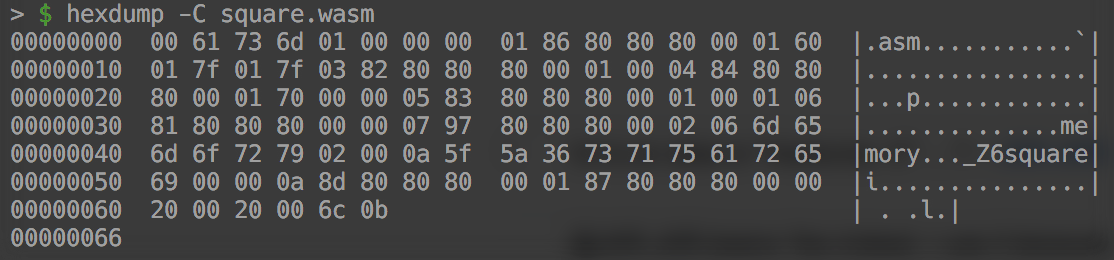
\includegraphics[width=14cm]{images/image-9}}
    }{
    \Fonte{Elaborada pelo autor.}
    \Nota{Imagem gerada utilizando a ferramenta \textit{hexdump} que exibe o conteúdo do
    arquivo utilizando notação hexadecimal.}
    }
\end{figure}

O último passo do processamento é carregar o módulo e executar a função \textit{square}.
Para isso será utilizado o código descrito no Código-fonte \ref{alg:code-5} que é
responsável por carregar, compilar e instânciar o módulo referente a essa função.

\lstinputlisting[language=JavaScript,caption={\label{alg:code-5} Carregamento e execução da função \textit{square}}]{code/load_module.js}

Na linha 1 é utilizada a função "fetch" fornecida pelo motor \textit{JavaScript} que
carrega o arquivo descrito, neste exemplo seria "square.wasm", e retorna um
\textit{promise} com o resultado. Na linha 2, é feita a leitura do conteúdo do arquivo e
é retornado um novo \textit{promise} com o conteúdo na forma de um vetor de
\textit{bytes}. Na linha 3, é utilizada a função \textit{instantiate} do objeto
\textit{WebAssembly} fornecida pelo motor \textit{JavaScript}, que compila o código
fornecido para código de máquina e retorna um objeto com dois campos, sendo o primeiro
campo o módulo representando o módulo \textit{WebAssembly} compilado e o segundo campo
sendo uma instância desse módulo que contém todas as funções exportadas por esse mesmo
módulo \textit{WebAssembly}. Vale ressaltar que nessa etapa podem ser lançadas exceções
caso ocorra algo inesperado durante a compilação, um exemplo disso pode ser
erros de tipo. Nas linhas 5 e 6, é utilizado o campo \textit{exports} da instância do
módulo que contém todas as funções exportadas e é executada a função \textit{square}.
Após o final da execução o valor 100 é exibido no \textit{console} do navegador, através
da função \textit{log} do objeto \textit{console} fornecida pelo motor
\textit{JavaScript}.